\usetikzlibrary{arrows.meta,calc}
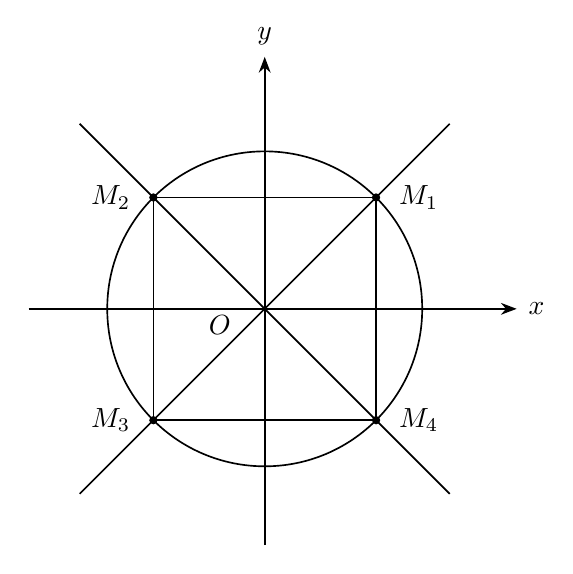
\begin{tikzpicture}[x=1cm,y=1cm,line width=.6pt,font=\normalsize,every node/.style={inner sep=0pt},>=Stealth]
\coordinate (O) at (0,0);
\coordinate (M1) at (1.414213562373,1.414213562373);
\coordinate (M2) at (-1.414213562373,1.414213562373);
\coordinate (M3) at (-1.414213562373,-1.414213562373);
\coordinate (M4) at (1.414213562373,-1.414213562373);
\draw[->] (-3.0,0)--(3.2,0) node[anchor=west,inner sep=0pt,xshift=4pt] {$x$};
\draw[->] (0,-3.0)--(0,3.2) node[anchor=south,inner sep=0pt,yshift=4pt] {$y$};
\draw (-2.35,-2.35)--(2.35,2.35);
\draw (-2.35,2.35)--(2.35,-2.35);
\draw (M1)--(M2)--(M3)--(M4)--cycle;
\draw (0,0) circle[radius=2.0cm];
\fill (M1) circle[radius=1.5pt];
\fill (M2) circle[radius=1.5pt];
\fill (M3) circle[radius=1.5pt];
\fill (M4) circle[radius=1.5pt];
\node[anchor=north east,inner sep=0pt,xshift=-12pt,yshift=-2pt] at (O) {$O$};
\node[anchor=west,inner sep=0pt,xshift=8pt] at (M1) {$M_{1}$};
\node[anchor=east,inner sep=0pt,xshift=-8pt] at (M2) {$M_{2}$};
\node[anchor=east,inner sep=0pt,xshift=-8pt] at (M3) {$M_{3}$};
\node[anchor=west,inner sep=0pt,xshift=8pt] at (M4) {$M_{4}$};
\end{tikzpicture}
